%-------------------------------------------------------------------------
\section{Non-isothermal compressible flow - HT process}
\label{sec:nonisothermal_gas_flow}

\subsection{Theory}

For non-isothermal flow we have to account for temperature changes
in the ideal gas law (\ref{eqn:ideal_gas_law}). 
%
\begin{equation}
\frac{\p\rho}{\p t}
=
\frac{\p}{\p t}
\left(
\frac{p}{R_{\mbox{\small air}}T}
\right)
=
\frac{1}{R_{\mbox{\small air}}T}
\frac{\p p}{\p t}
-
\frac{p}{R_{\mbox{\small air}}T^2}
\frac{\p T}{\p t}
\end{equation}

%Aux step
%\begin{equation}
%\nabla(\frac{p}{T}\nabla p)
%=
%\frac{1}{2}
%\nabla(\frac{1}{T}\nabla p^2)
%=
%\frac{1}{2}
%\left(
%-\frac{1}{T^2}\nabla T \nabla p^2
%+
%\frac{2p}{T}\Delta p
%\right)
%=
%-\frac{p}{T^2}\nabla T \nabla p
%+
%\frac{p}{T}\Delta p
%\end{equation}

The fluid
mass balance equation is then given by
%
\begin{equation}
n
\frac{1}{T}
\frac{\p p}{\p t}
-
n
\frac{p}{T^2}
\frac{\p T}{\p t}
-
\nabla
\cdot
\left(
\frac{p}{T}
\frac{\PermTensor}{\mu}
\nabla p
\right)
=
R_{\mbox{\small air}} Q_\rho
\label{eqn:fluid_mass}
\end{equation}

%-------------------------------------------------------------------------
%\subsection{Heat transport}
%
For heat transport there is an advective term due to air flow. 
The heat transport equation is as follows.
%
\begin{equation}
c\rho
\frac{\p T}{\p t}
+
c^g\rho^g
n\VelocityVector^g
\cdot
\nabla T
-
\nabla\cdot\left[\lambda\nabla T\right]
=
Q_T
\label{eqn:heat_transport}
\end{equation}
%
with $c\rho=n(c^g\rho^g)+(1-n)c^s\rho^s$, heat
capacity of porous medium and
$\lambda=n \lambda^g +(1-n)\lambda^s$, heat
conductivity of porous medium. Superscripts $g,s$ denote gas and solid phases of the
porous medium, respectively. Using the ideal gas law
(\ref{eqn:ideal_gas_law}), density of the porous medium is given
by
%
\begin{equation}
\rho
=
n \frac{p}{R_{\mbox{\small air}}T}
+
+
(1-n)\rho^s
\end{equation}
%

%-------------------------------------------------------------------------
\subsection{Material functions}
\label{sec:materials}

For non-isothermal air flow and heat transport we have to consider
in addition to the ideal gas law (\ref{eqn:ideal_gas_law}) the
pressure and temperature dependencies of air viscosity
$\mu^g(p,T)$ (section \ref{sec:viscosity}), specific heat
capacities $c^g(p,T)$ and heat
conductivities $\lambda^g(p,T)$ (section
\ref{sec:thermal_properties}) as well (\cite{McDermottEtAl:2006}).

\subsubsection{Air viscosity}
\label{sec:viscosity}

The Reichenberg viscosity model (\cite{ReidEtAl:1988}) is used for the
non-isothermal flow of air. The pressure and temperature
dependencies of air viscosity are shown in Fig. \ref{fig:visco7}.
%
\begin{eqnarray}
\Viscosity^g (\Pressure,\Temperature)
=
\Viscosity_0 (T)
\left(
1 + \frac{A\Pressure_r^{3/2}}{B\Pressure_r+(1+C\Pressure_r^D)^{-1}}
\right)
\label{eqn:reichenberg_viscosity}
\end{eqnarray}
%
with the following parameters:
\begin{eqnarray}
\begin{array}{ll}
\Pressure_r = \Pressure / \Pressure_{\mbox{\footnotesize crit}}
&
\Temperature_r = \Temperature / \Temperature_{\mbox{\footnotesize crit}}
\\
A = \D\frac{\alpha_1}{T_r} \exp (\alpha_2 T_r^a)
&
B = A(\beta_1 T_r - \beta_2)
\\
C = \D\frac{\gamma_1}{T_r} \exp (\gamma_2 T_r^c)
&
D = \D\frac{\delta_1}{T_r} \exp (\delta_2 T_r^d)
\end{array}
\\
\begin{array}{lll}
\Pressure_{\mbox{\footnotesize crit}} = 33.9 \times 10^4 \, Pa
&
\Temperature_{\mbox{\footnotesize crit}} = 126.2 \, K
\\
\alpha_1 = 1.9824\times 10^{-3}  &  \alpha_2 = 5.2683  &  a = -0.5767 \\
\beta_1  = 1.6552               &  \beta_2  = 1.2760  &  \\
\gamma_1 = 0.1319                &  \gamma_2 = 3.7035  &  c = -79.8678 \\
\delta_1 = 2.9496                &  \delta_2 = 2.9190  &  d = -16.6169
\end{array}
\nonumber
\end{eqnarray}

% *** EPS-Grafik ***
\begin{figure}[htb!]
\begin{center}
\footnotesize
%\psfrag{Synonym}[pos][pos]{Tex-Ersetzung}
%\psfrag{x}[][]{$t$}
%\psfrag{y}[b][t]{$y(t)$}
%\psfrag{t}[][]{ }
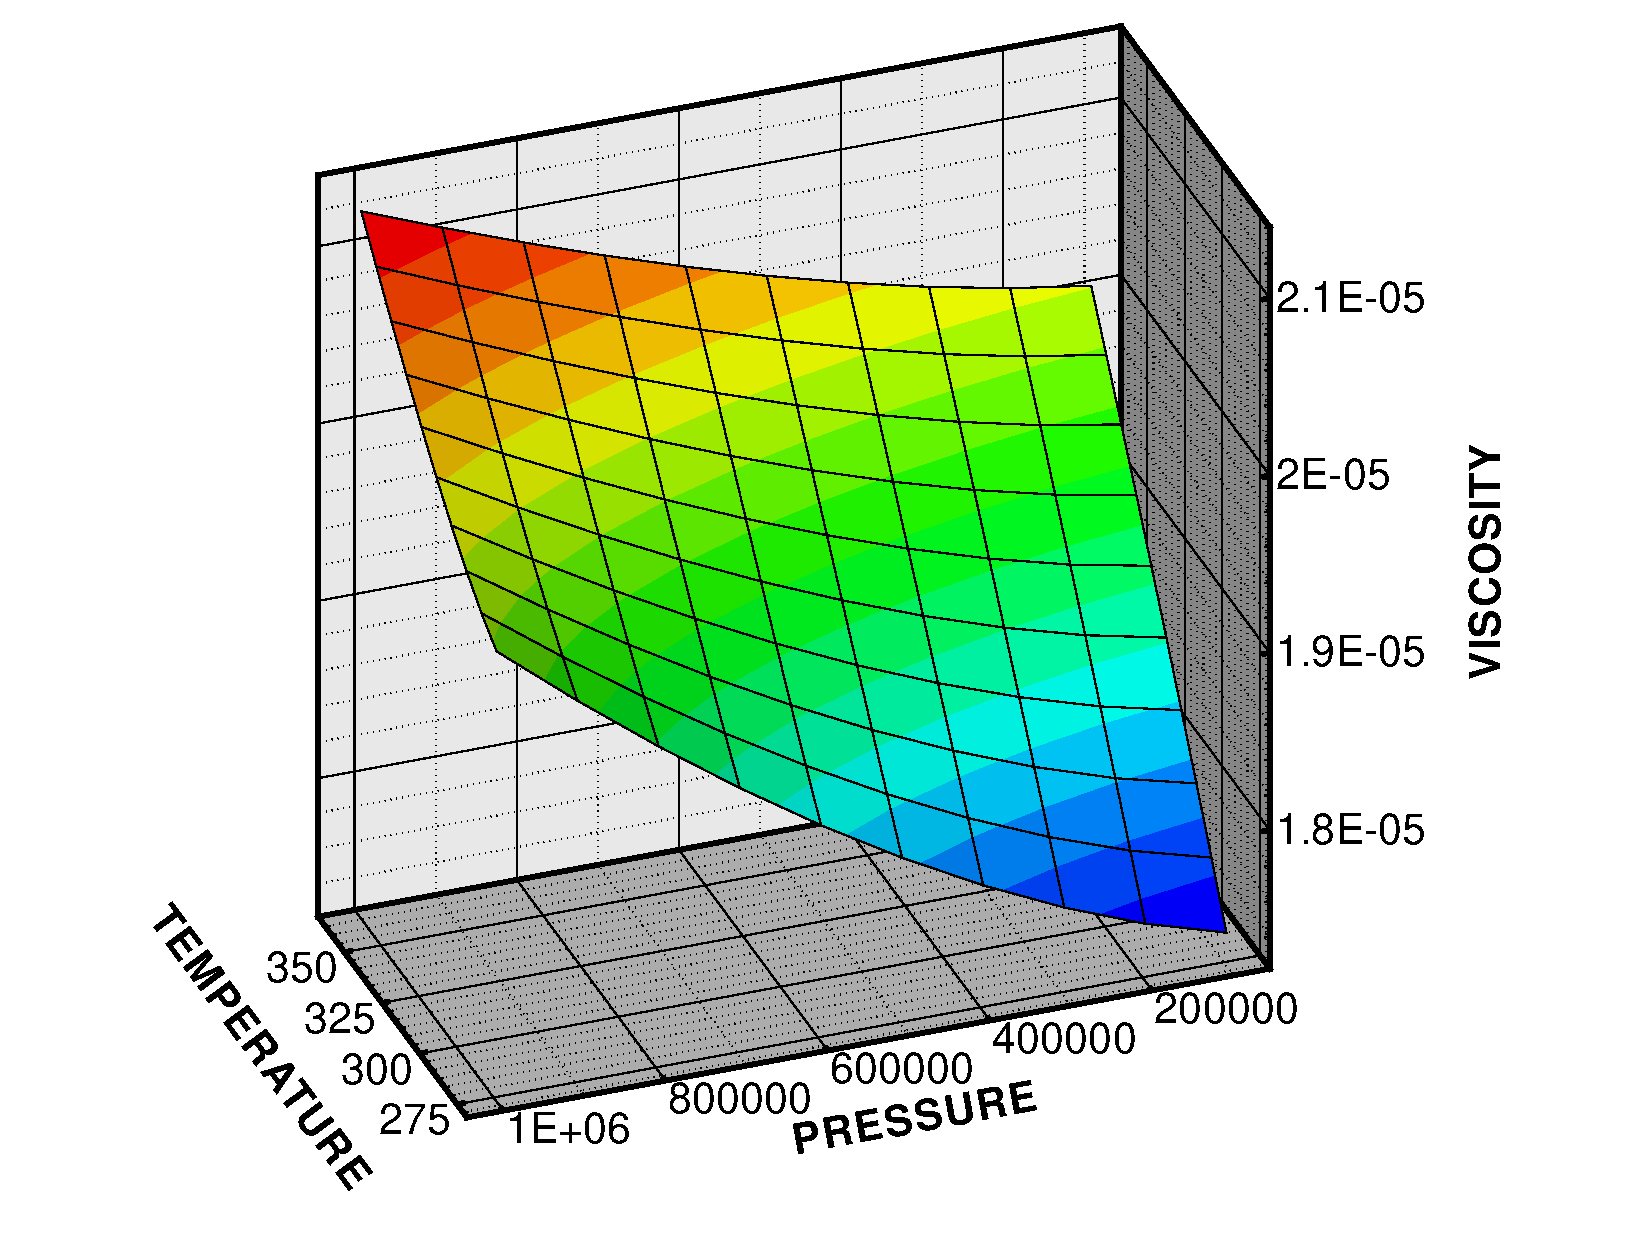
\includegraphics[width=0.85\columnwidth]{H_GAS/figures/viscosity.eps}  % Filename.eps
\caption{Air viscosity as a function of temperature (in Kelvin) and pressure (in Pa)}
\label{fig:visco7}
\end{center}
\end{figure}
%

\subsubsection{Thermal properties}
\label{sec:thermal_properties}

Beside the hydraulic characteristics such as air viscosity, the thermal properties of the gas and solid, such as heat capacity and thermal conductivity are important for heat transport.
As an example, Fig. \ref{fig:thermal_properties} depicts the thermal properties of the gaseous phase.
Fig. \ref{fig:thermal_properties} (left) shows the temperature dependence of specific heat capacity of air at atmospheric pressure corresponding to equation (\ref{eqn:heat_capacity}) from \cite{ZografosEtAl:1987} and compared with experimental data by \cite{VargaftikEtAl:1996}. Fig. \ref{fig:thermal_properties} (right) illustrates the temperature dependence of thermal conductivity of air at atmospheric pressure corresponding to equation (\ref{eqn:thermal_conductivity}) from \cite{ZografosEtAl:1987}  and compared with experimental data by \cite{VargaftikEtAl:1996}. The pressure dependency of thermal properties can be neglected in the present pressure regimes.

\begin{eqnarray}
c^g
=
1.0613
-
4.3282 \times 10^{-4} T
+
1.0234 \times 10^{-6} T^2
-
6.4747 \times 10^{-10} T^3
\nonumber
\\
+
1.3864 \times 10^{-13} T^4
\label{eqn:heat_capacity}
\end{eqnarray}

\begin{eqnarray}
\lambda^g
=
7.488 \times 10^{-3}
-
1.7082 \times 10^{-4} T
+
2.3758 \times 10^{-7} T^2
-
2.2012 \times 10^{-10} T^3
\nonumber
\\
+
9.46 \times 10^{-14} T^4
-
1.579 \times 10^{-17} T^5
\nonumber
\\
\label{eqn:thermal_conductivity}
\end{eqnarray}

%-----------------------------------------
\newpage
\begin{figure}[htb!]
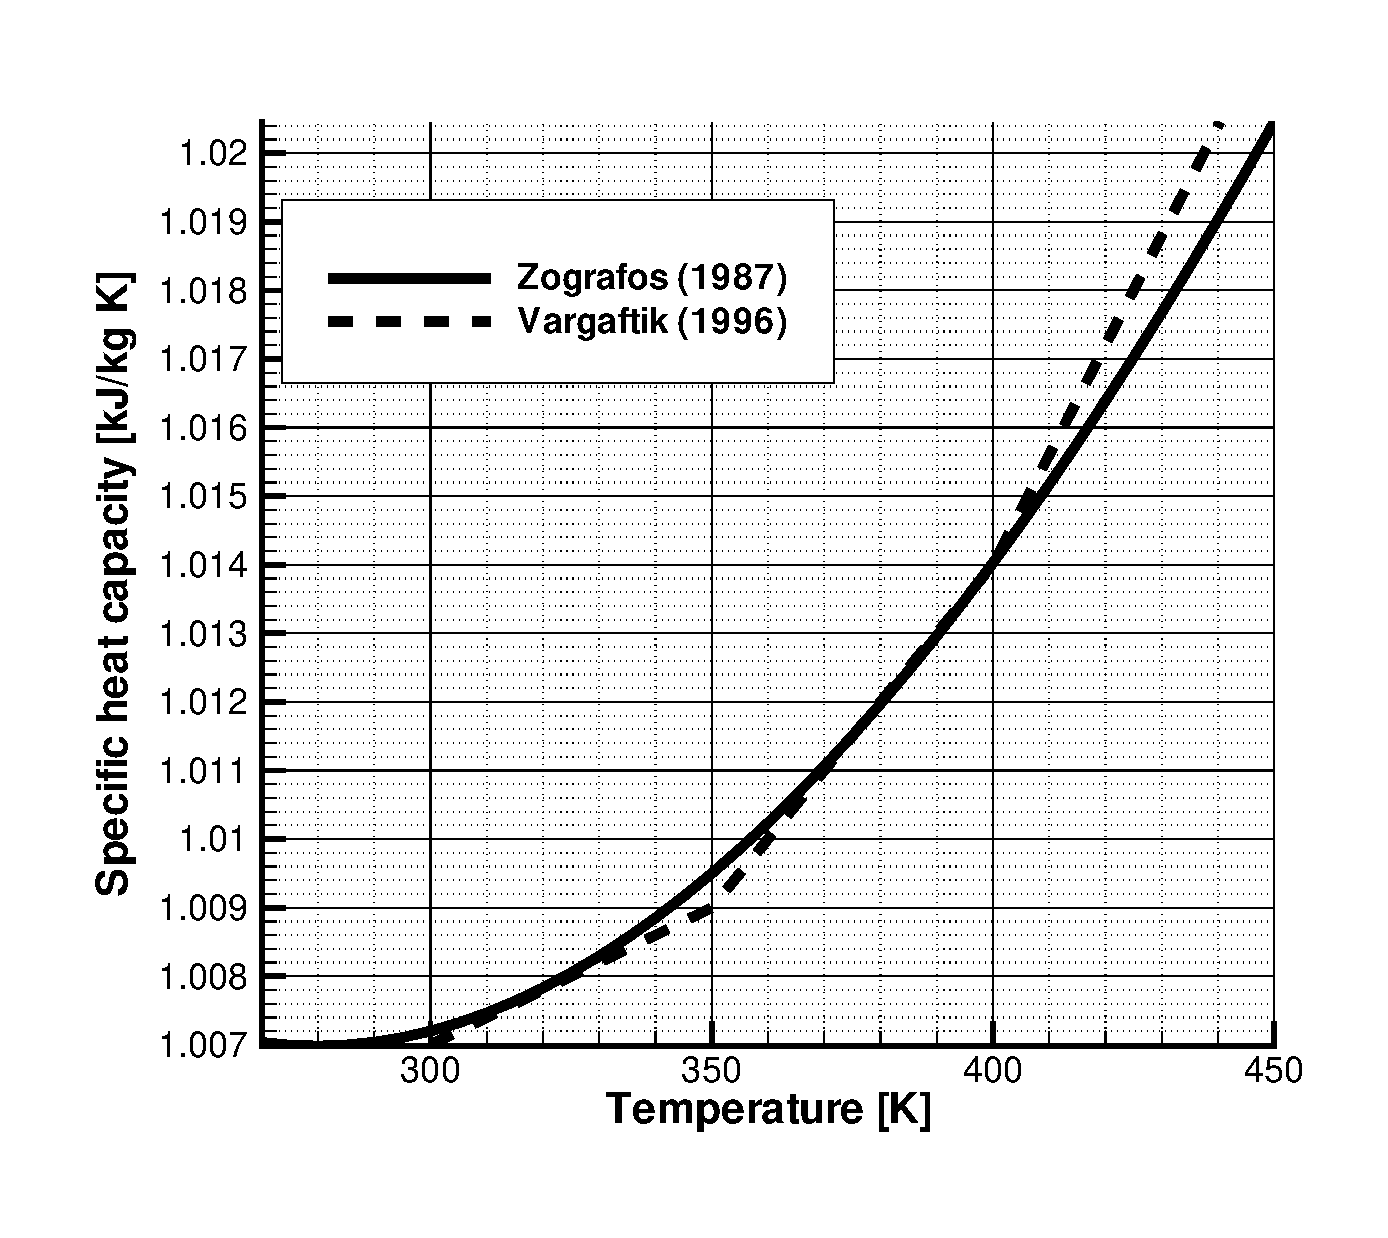
\includegraphics[scale=0.4]{H_GAS/figures/heat_capacity_air.eps}
\end{figure} 
\begin{figure}[htb!]
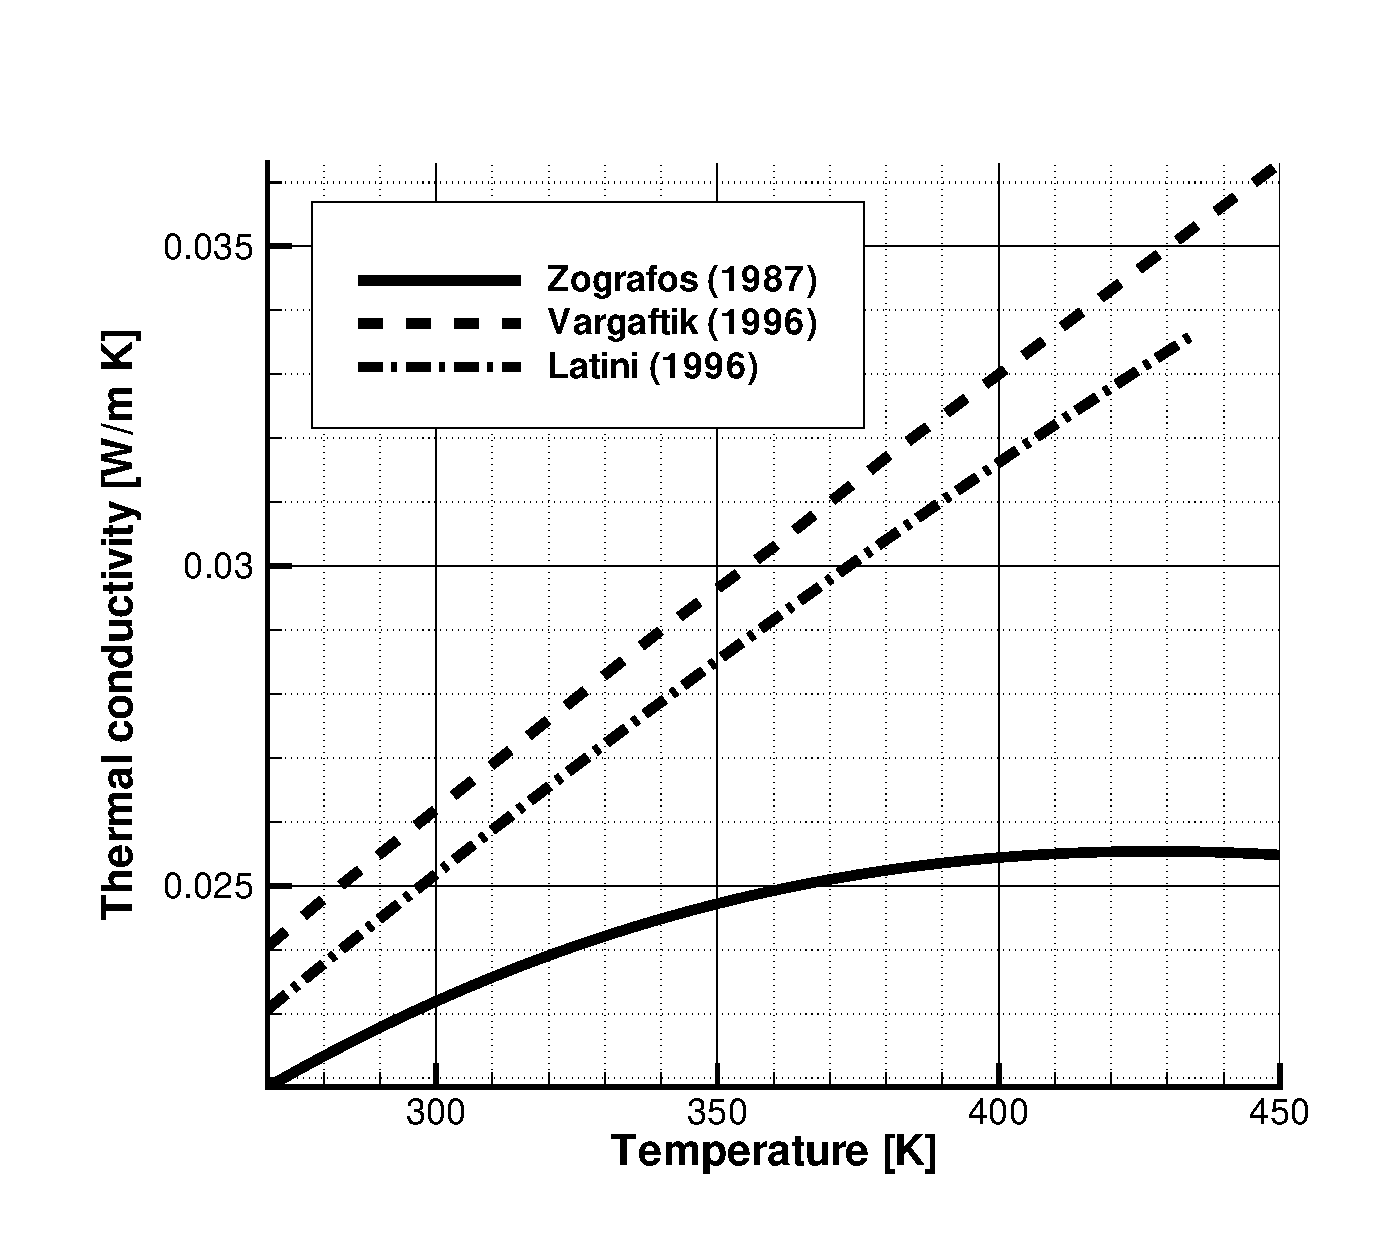
\includegraphics[scale=0.4]{H_GAS/figures/heat_conductivity_air.eps}
\caption{Thermal properties of air: Heat capacity (top), thermal conductivity (bottom)}
\label{fig:thermal_properties}
\end{figure} 

%-----------------------------------------
\newpage
\begin{figure}[htb!]
\includegraphics[scale=0.4]{H_GAS/figures/press_ply.eps}
\end{figure}
\begin{figure}[htb!]
\includegraphics[scale=0.4]{H_GAS/figures/velo_ply.eps}
\caption{Hydraulic profiles evolution: Air pressure (top), Air velocity (bottom)}
\label{fig:air_flow}
\end{figure}

\newpage
\subsection{Examples}

\subsubsection{Air flow}

We consider the same test example definition as for isothermal gas flow in sec. \ref{sec:h_gas}.
Now we use temperature dependent fluid properties according to the Reichenberg model described in section \ref{sec:materials}.
The model parameters are summarized in Tab. \ref{tab:air_heat_1d}.

\begin{table}[!htb]
\centering
\begin{tabular}{llll}
\hline\hline\noalign{\smallskip}
Property & Symbol & Value & Unit \\
\noalign{\smallskip}\hline\noalign{\smallskip}
Model length & $L$ & $100$ & $m$\\
Cross section area & $A$ & $1$  & $m^2$ \\
Porosity & $n$ & $0.35$  & $-$ \\
Densities & $\rho^g,\rho^s$ & (\ref{eqn:ideal_gas_law}),$2650$ & $kg/m^3$ \\
\hline
Permeability & $k$ & $2.7\times 10^{-11}$ & $m^2$\\
Dynamic gas viscosity & $\mu$ & (\ref{eqn:reichenberg_viscosity}) & $Pa\,s$\\
Initial condition & $p_I$ & $101325$ & $Pa$\\
Boundary condition & $p_1$ & $101325$ & $Pa$\\
Injection rates & $Q^p$ & $1-10$ & $kg/s$\\
\hline
Heat dispersion length & $\alpha_L,\alpha_T$ & $1,0.1$ & $m$\\
Heat conductivities & $\lambda^g,\lambda^s$ & (\ref{eqn:thermal_conductivity}), $2.5$ & $W/(m K)$\\
Heat capacities & $c^g,c^s$ & (\ref{eqn:heat_capacity}), $2300$ & $J/(kg K)$\\
\hline
Time step & $\Delta t$ & $10^4$ & $s$\\
Space step & $\Delta x$ & $1$ & $m$\\
\noalign{\smallskip}\hline\hline
\end{tabular}
\caption{Model parameters}
\label{tab:air_heat_1d}
\end{table}

Fig. \ref{fig:air_flow} show the air pressure (left) and velocity
distributions (right) along the soil profile. Simulations were run with
constant viscosities and those corresponding to the Reichenberg
model (section \ref{sec:viscosity}) which takes pressure and
temperature changes into account.

\begin{figure}[htb!]
%\begin{center}
%\begin{minipage}[t]{0.45\textwidth}
%\begin{center}
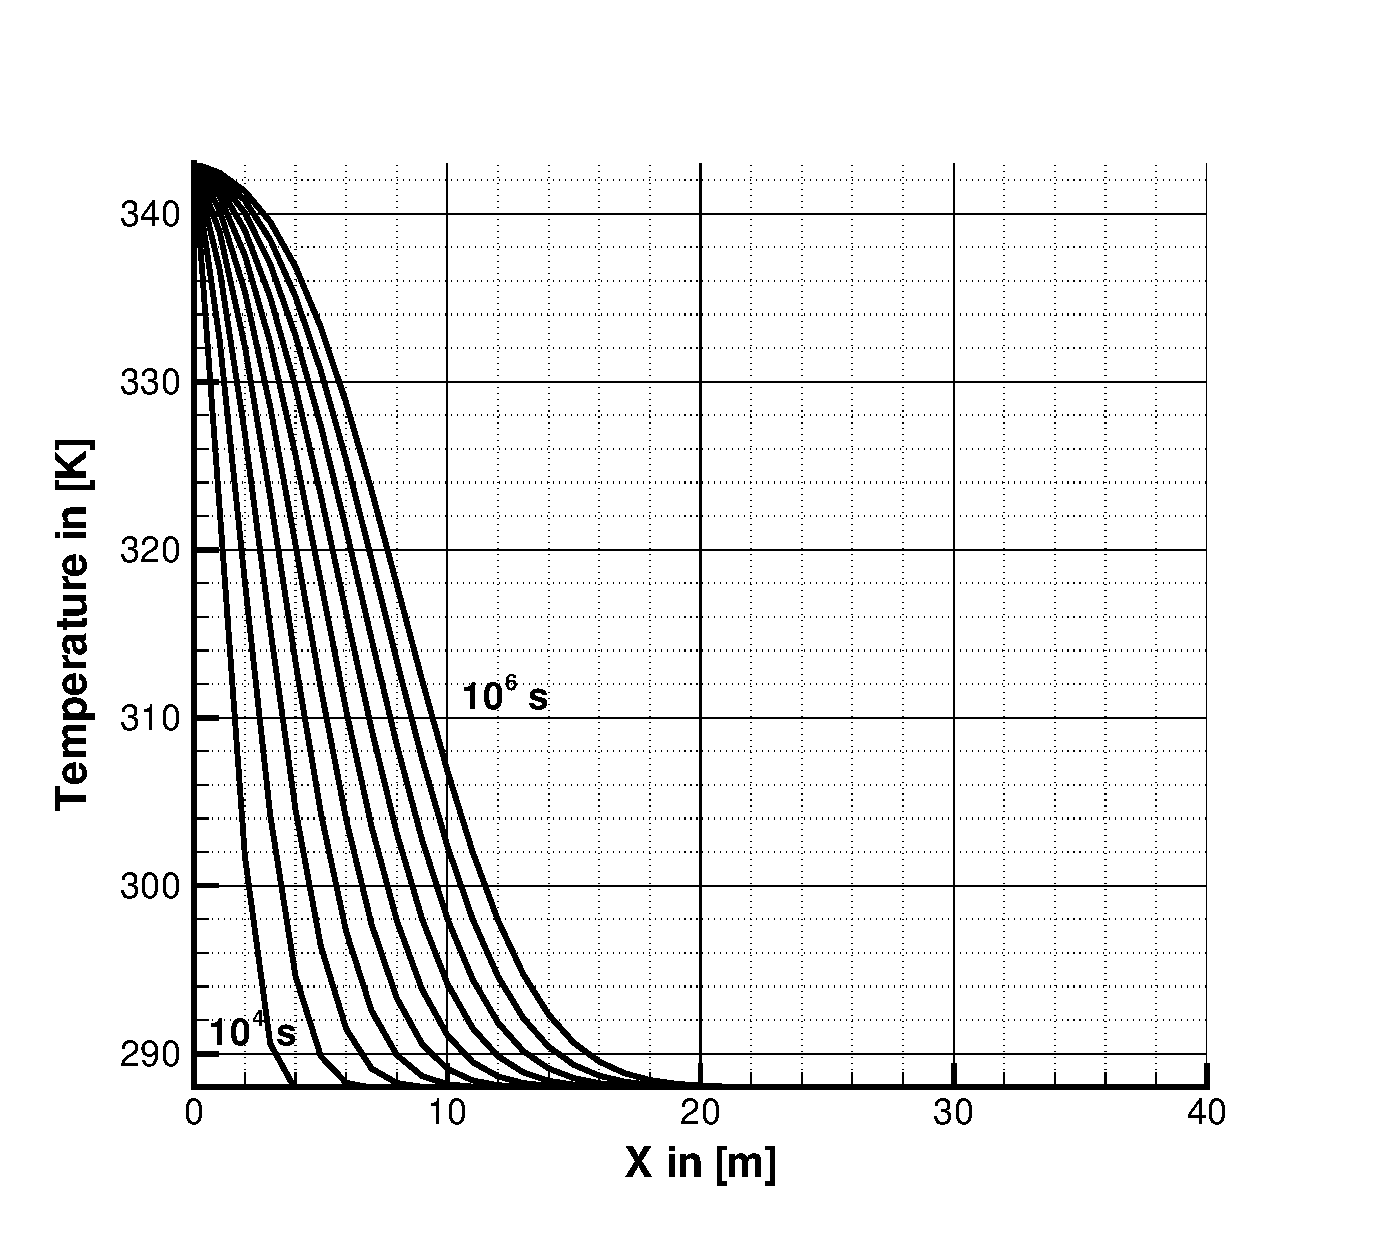
\includegraphics[scale=0.4]{H_GAS/figures/t_1.eps}\\
%\centerline{$1 kg/s$ air injection rate}
%\end{center}
%\end{minipage}
%\hspace{0.07\textwidth}
%\begin{minipage}[t]{0.45\textwidth}
%\begin{center}
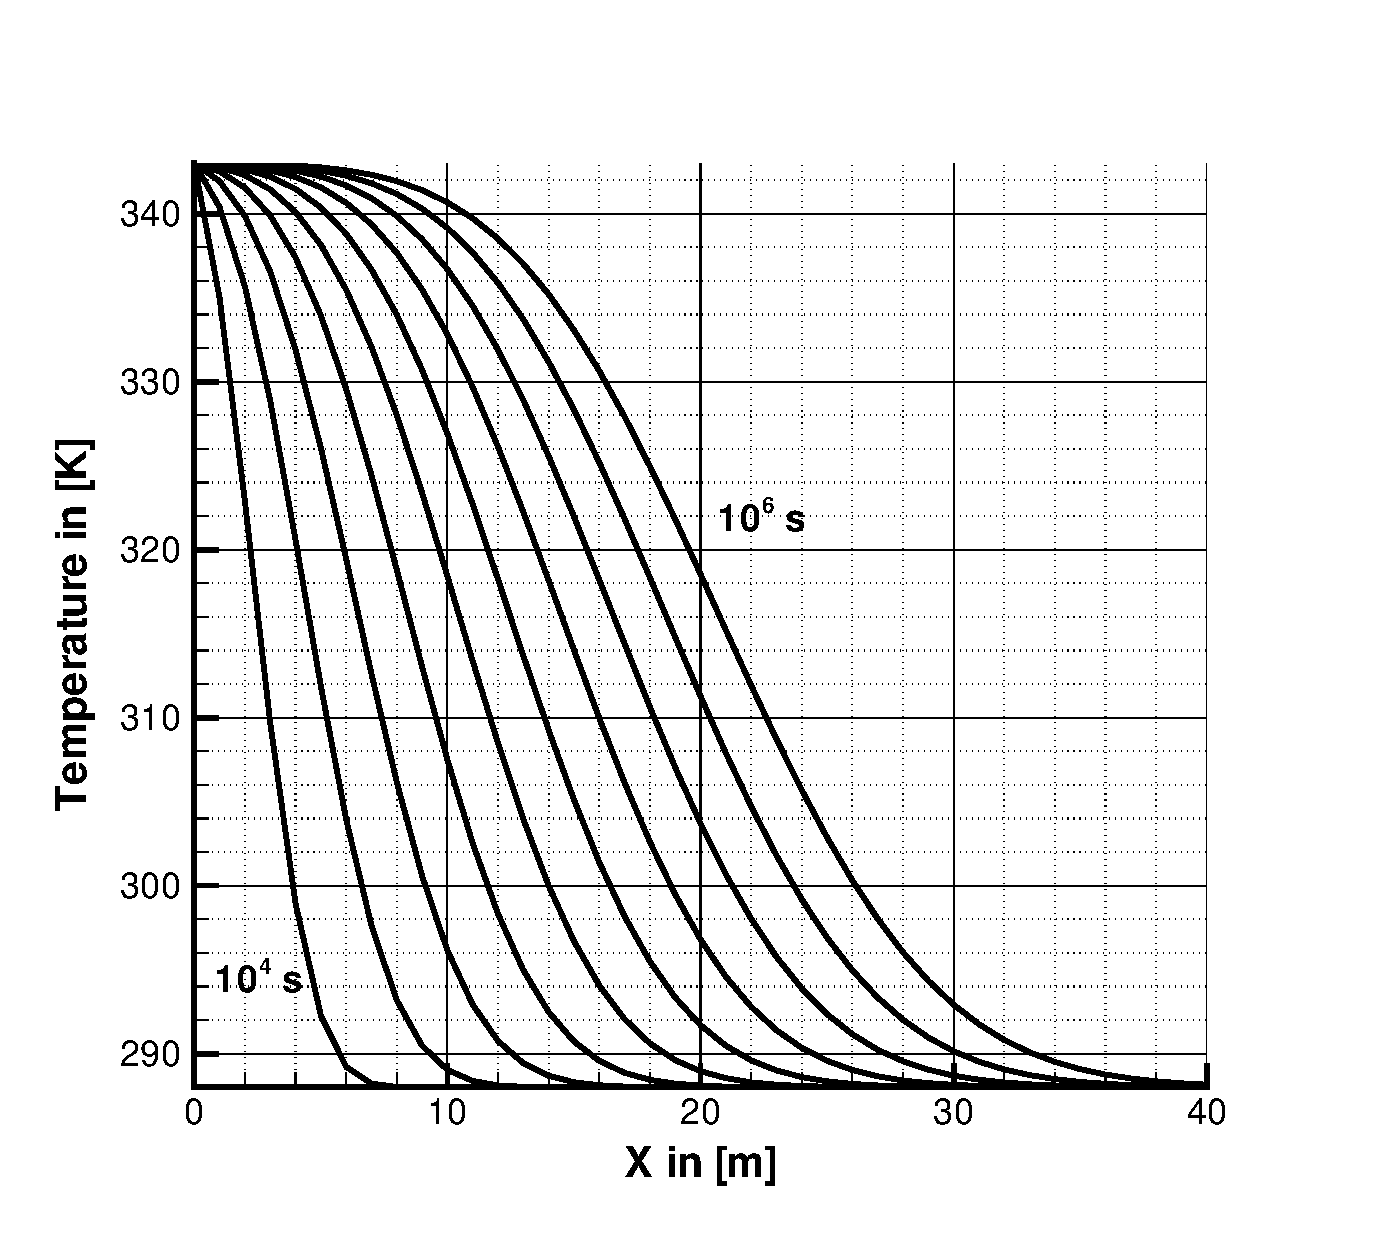
\includegraphics[scale=0.4]{H_GAS/figures/t_10.eps}\\
%\centerline{$10 kg/s$ air injection rate}
%\end{center}
%\end{minipage}\\
%\end{center}
\caption{Air temperature profiles evolution. $1 kg/s$ air injection rate (top), $10 kg/s$ air injection rate (bottom)}
\label{fig:air_heat_1d_heat}
\end{figure}

The corresponding temperature profiles for different air injection rates are depicted in Fig. \ref{fig:air_heat_1d_heat}. The different shapes of the thermal profile curves indicate the transition between diffusion (left) and advection dominated regimes (right).
%
Fig. \ref{fig:visco8} shows the temporal evolution of air pressure profiles for non-isothermal gas flow. In order to see the non-isothermal effects we plotted the analytical steady state solution for isothermal flow along with present numerical solution for non-isothermal flow. As a consequence of the viscosity increase resulting from the Reichenberg model the steady state pressure is larger for non-isothermal conditions.

\begin{figure}[htb!]
\begin{center}
\footnotesize
\includegraphics[width=0.85\columnwidth]{H_GAS/figures/non_isothermal_flow.eps}  % Filename.eps
\caption{Temporal evolution of air pressure profiles for non-isothermal gas flow}
\label{fig:visco8}
\end{center}
\end{figure}

\subsubsection*{Benchmark repository}
\begin{tabular}{|l|l|l|l|}
\hline
Problem type & Repository path & Files & Version \\
\hline
\verb H_GAS & \verb benchmarks\h_gas\nonisothermal_gas_flow & \verb h_gas_line & 4.4.04(OK) \\
\hline
\end{tabular}

%\subsubsection{\CO2 flow}
\clearpage
\newpage

\section{Joule-Thomson process in permeable media - HT process}
\label{sec:JTProcesses}
\subsubsection*{\upshape\textbf{Theory}}
Flow in permeable media is not an isothermal process because there is a temperature change resulting from fluid expansion and viscous dissipation heating. Interests of this problem is to use the energy balance equation with heat transfer related with expansion and viscous dissipation for prediction of temperature profiles. For gas phase with only one component as carbon dioxide, we can start from the thermal energy balance as the following form
\begin{equation}
\left(\rho c_p\right)_{\mathrm {eff}} \frac{\partial T}{\partial t} + c_p^g \rho^g \mathbf u \cdot \nabla T - \nabla \cdot \left[\kappa_{\mathrm {eff}} \nabla T\right] = n \beta_{\mathrm T} T \frac{\partial p}{\partial t} + \left(\beta_{\mathrm T} T-1\right) \mathbf u \cdot \nabla p + Q_T
\label{eq:EnergyBalance}
\end{equation}
In the following we develop an analytical solution for one-dimensional (\textbf{1D}) steady energy balance equation.
The pressure relationship is described by Darcy law as:
\begin{equation}
u_{\mathrm x}=-\frac{\mathbf k}{\mu} \frac{\partial p}{\partial {\mathrm x}}
\label{eq:DarcyVelocity}
\end{equation}
In a one-dimensional Cartesian coordinate (x-direction), steady energy balance becomes
\begin{equation}
c_p^g\rho^g u_{\mathrm x}\frac{\partial T}{\partial {\mathrm x}}- \beta_{\mathrm T} T u_{\mathrm x} \frac{\partial p}{\partial {\mathrm x}}+u_{\mathrm x} \frac{\partial p}{\partial {\mathrm x}}- \kappa_{\mathrm {eff} }\frac{\partial^2 T}{\partial {\mathrm x}^2} =0
\label{eq:SteadyEnergyBalance}
\end{equation}
Substituting Eq. (\ref{eq:DarcyVelocity}) into Eq.(\ref{eq:SteadyEnergyBalance}) and rearranging give
\begin{equation}
\frac{\partial^2 T}{\partial {\mathrm x}^2}-\frac{c_p^g\rho^g}{\kappa_{\mathrm {eff} }} u_{\mathrm x}\frac{\partial T}{\partial {\mathrm x}}- \frac{\mu \beta_{\mathrm T}}{\mathbf k \kappa_{\mathrm {eff} }} u^2_{\mathrm x} T + \frac{\mu }{\mathbf k \kappa_{\mathrm {eff} }} u^2_{\mathrm x} =0
\label{eq:SOSteadyEnergyBalance}
\end{equation}
Solving the second order ordinary differential equation (\ref{eq:SOSteadyEnergyBalance}) gives
\begin{equation}
T=L_+\exp(m_+~\mathrm x)+L_-\exp(m_-~\mathrm x)+\frac{1}{\beta_{\mathrm T}}
\label{eq:AnlyticalSolution}
\end{equation}
where 
\begin{equation*}
m_{\pm}=u_{\mathrm x}\left(\frac{c_p^g\rho^g}{\kappa_{\mathrm {eff} }}\pm\sqrt{\left(\frac{c_p^g\rho^g}{\kappa_{\mathrm {eff} }}\right)^2 + \frac{4\beta_{\mathrm T}\mu}{\mathbf k \kappa_{\mathrm {eff} }}} \right)
\label{eq:AnlyticalSolution}
\end{equation*}
 and $\mathrm {L_+}$ and $\mathrm {L_-}$ are integration constants to be determined by boundary conditions.
 
 
\subsubsection*{\upshape\textbf{Problem definition}}
The test benchmark problem for Joule-Thomson cooling processes has been solved. Problem is formulated for the expansion occurs during injection of compressed cryogenic $\mathrm {CO_2}$ in a one-dimensional (\textbf{1-D}) horizontal column. We assume that column is a permeable media which is filed with $\mathrm {CO_2}$ at low pressure. Finite element solution has been obtained through solving the mass and energy balance equations. Within a time step mass balance equation for pressure is solved with temperature changes in return the energy balance equation, i.e. Eq. (\ref{eq:EnergyBalance}) is then solved for temperature with obtained fluid velocity. This is so called staggered approach and executed until solution become steady. Model geometry and conditions has shown in Fig. \ref{fig:JTGeometry}\\
\begin{figure}[htb!]
\vspace{-0.25in}
\centering
\includegraphics[width=1.0\textwidth]{H_GAS/figures/JTCoolingGemetry.eps}
\vspace{-0.7in}
\caption{Model geometry and conditions}
\label{fig:JTGeometry}
\end{figure}
\vspace{-0.25in}
\subsubsection*{\upshape\textbf{Results}}
Based on the above discussion OpenGeoSys (OGS) capable to show the Joule-Thomson process in carbon sequestration with enhanced gas recovery (CSEGR) related problems. In Fig. \ref{fig:JTComparison} we have presented comparison of temperature profile produced from OGS with those of analytical solution, i.e. Eq. (\ref{eq:AnlyticalSolution}). In this figure `\textbf{without solid matrix}' mean the case where we do not account heat provide by solid matrix by setting $c_p^s=0, \kappa^s=0$ whereas case `\textbf{with solid matrix}' mean we have accounted heat provided by solid matrix.
\begin{figure}[htb!]
\centering
\includegraphics[width=0.75\textwidth]{H_GAS/figures/JTCooling.eps}
\caption{Comparison of present solution (FEM) with analytical solution due to Eq. (\ref{eq:AnlyticalSolution}).}
\label{fig:JTComparison}
\end{figure}
The physical domain has been discretized in hundred line element which size is varying between $\delta {\mathrm x}=0.4~\mathrm m$ to $\delta {\mathrm x} = 4.3498~\mathrm m$. This helps to capture the sharp gradient of temperature present near the injection point. Concerning to the time step size, at beginning of the simulation $\delta t=1~\mathrm s$ with step by step increasing it reaches to $\delta t=9.0\times10^4~\mathrm s$ ofter $14$ time steps.


Figure shows that as we inject $\mathrm {CO_2}$ (at temperature $120^{\circ}$C which is lower than inversion temperature $\approx 1227^{\circ}$C), its pressure falls with high gradient. It means as expansion starts, the average distance between molecules grows. Because of intermolecular attractive forces, expansion causes an increase in the potential energy of the gas. As no external work is extracted and process is adiabatic, the total energy of the gas remains constant because of the conservation of energy. The increase in potential energy thus implies a decrease in kinetic energy and therefore temperature falls.
\begin{table}[htbp]
\caption{Model parameters}
\label{tab:Material_parameters}\begin{tabular}{l*{3}{l}l}
\hline
Meaning & Symbol & Value \\ 
\hline
Column radius & $L$ & $100~(\mathrm {m})$\\
Porosity & $n$ & $0.35~(-)$ \\
Densities & $\rho^g,\rho^s$ & $\frac{p M}{z_{\mathrm {sc}} R T}, 2460~(\mathrm {kg~m^{-3}})$\\
Permeability & $\textbf{k}$ & $2.7\times 10^{-11}~(\mathrm {m^2})$\\
Dynamic viscosity & $\mu$ & $1.9836\times10^{-5}~(\mathrm {Pa~s})$\\
Heat conductivities & $\kappa^g,\kappa^s$ & $0.02.6374, 2.5~(\mathrm {W~m^{-1} K^{-1}})$\\
Heat capacities & $c_p^g,c_p^s$ & $1.067\times10^3, 1.2\times10^3 (\mathrm {J kg^{-1} K^{-1}})$\\
\hline
\end{tabular}
\end{table}

\subsubsection*{\upshape\textbf{Benchmark deposit}}
\begin{tabular}{|l|l|l|}
\hline
Benchmark & Problem type & Path in benchmark deposit \\
\hline
JTCooling& H-GAS & JT-Cooling \\
\hline
\end{tabular}
\clearpage

